%%%%%%%%%%%%%%%%%%%%%%%%%%%%%%%%%%%%%%%%%%%%%%%%%%
%% Bachelor's & Master's Thesis Template        %%
%% Copyleft by Dawid Weiss & Marta Szachniuk    %%
%% Faculty of Computing and Telecommunication   %%
%% Poznan University of Technology, 2020        %%
%%%%%%%%%%%%%%%%%%%%%%%%%%%%%%%%%%%%%%%%%%%%%%%%%%

% Szkielet dla pracy Magisterskiej pisanej w języku polskim.

\documentclass[polish,a4paper,oneside]{ppfcmthesis}
\pagenumbering{arabic}

\usepackage[utf8]{inputenc}
\usepackage[OT4]{fontenc}
\usepackage{float}
\usepackage[inkscapelatex=false]{svg}
\usepackage{geometry}
\usepackage{graphicx}
\usepackage{tocloft}


%--------------------------------------
% Strona tytułowa
%--------------------------------------

% Autorzy pracy, jeśli jest ich więcej niż jeden
% wstaw między nimi separator \and
\author{% 
    Jan Biały \album{144334}}
\authortitle{inż.}

\title{Zarządzanie przydziałem zasobów w środowisku Metaverse}

% Your supervisor comes here.
\ppsupervisor{prof.~dr hab.~inż.~Anna Kobusińska} 

% Year of final submission (not graduation!)
\ppyear{2024}                                 

\begin{document}
\pagestyle{ppfcmthesis}%

% Front matter starts here
\pagestyle{empty}%
\maketitle\cleardoublepage%

%--------------------------------------
% Miejsce na kartę pracy dyplomowej
%--------------------------------------

\thispagestyle{empty}\vspace*{\fill}%
\begin{center}Tutaj będzie karta pracy dyplomowej;\\oryginał wstawiamy do wersji dla archiwum PP, w pozostałych kopiach wstawiamy ksero.\end{center}%
\vfill\cleardoublepage%

%--------------------------------------
% Spis treści
%--------------------------------------

\setcounter{tocdepth}{2}
\tableofcontents*
\cleardoublepage % Ensure TOC ends and we start fresh

%--------------------------------------
% Rozdziały
%--------------------------------------

% Reset the page numbering to Arabic numerals for the main content
\pagestyle{ppfcmthesis}

\input{chapters/01-streszczenie_abstrakt}
\chapter{Wstęp}

\subsubsection{Kontekst}
\subsubsection{Cel pracy}

Podstawowym celem pracy jest stworzenie protokołu doboru zasobów do zapotrzebowania klienta w środowisku rozproszonym.

\subsubsection{Zawartość kolejnych rozdziałów}


\chapter{Podstawy teoretyczne}
\section{Metaverse}


Metaverse to koncepcja w świecie technologicznym, która odnosi się do cyfrowego środowiska życia w którym konwencjonalne struktury społeczne ulegają zmianie. Jest to termin, który łączy w sobie koncepcje greckiego prefiksu „meta”, który oznacza „pełniejszy” lub „przekraczający”, oraz akronimu „Verse” oznaczającego „wszechświat”, który oznacza pojemnik czasoprzestrzenny. Idea metawersji została wprowadzona w powieści science fiction Neala Stephensona \definicja{Snow Crash} w 1992 roku. Szybki rozwój technologii takich jak blockchain, wirtualna (\english{Virtual Reality}) i rozszerzona (\english{Augmented Reality}) rzeczywistość, gry, sztuczna inteligencja i Internet Rzeczy \acronym{IoT} (\english{Internet Of Things}) sprawiły, że metawersja stała się jednym z najbardziej popularnych terminów w świecie technologii. Rozwiązania i usługi są opracowywane dla wirtualnych światów, aby umożliwić użytkownikom dobrą zabawę, inteligentne angażowanie się w otoczenie i nawiązywanie głębszych relacji z innymi użytkownikami \cite{metaverseAsAService}. 

\begin{figure}[h!]
    \centering
    \includesvg[width=0.7\textwidth]{images/metaverse/MetaverseInfographic.svg}
    \caption{Koncepcyjny widok metaverse\cite{metaverseUseCaseslee}}
    \label{fig:enter-label}
\end{figure}

Metaverse jako wirtualny świat  wchodzący w interakcję ze światem rzeczywistym i śwaitem ludzkim. Interakcja ta została przedstawiona na ryskunku \ref{abstractMetaverseArchitectureHumanVirtualPhisical}. Metaverse jest uważany za idealne ucieleśnienie Internetu w przyszłości. Zintegrowany z zaawansowanymi technologiami, metawersja może być wirtualną przestrzenią wzbogaconą o rzeczywistość fizyczną. Użytkownicy są połączeni w wirtualnym wszechświecie we wciągającej interakcji i są ze sobą połączeni w celu prowadzenia działań społecznych. Odkąd koncepcja metaverse została zaproponowana w filmie naukowym \definicja{Snow Crash}, ludzie są stopniowo przyzwyczajają się do wirtualnych i internetowych aktywności zamiast w fizyczny i konwencjonalny sposób. Odkąd zaproponowano Przemysł 4.0, produkcja przemysłowa przekształca się w kierunku inteligentnej produkcji zwłaszcza w całym cyklu życia produktu, obejmującym badania i rozwój, produkcję, testy i eksperymenty, sprzedaż i transakcje oraz usługi i konserwację. Dzięki zaawansowanym technologiom informacyjno-komunikacyjnym, technologiom rozszerzonej rzeczywistości i sztucznej inteligencji, inteligentna produkcja jest wspierana przez wyższą wydajność produkcji i zwiększoną wirtualną interaktywność użytkowników. Ponadto, jako nowy paradygmat produkcji, produkcja w chmurze wygodnie zapewnia użytkownikom usługi na żądanie. Rozproszone zasoby produkcyjne są wirtualizowane i zarządzane w ujednolicony, zoptymalizowany i konfigurowalny sposób, umożliwiając wysoce wirtualną współpracę i innowacyjną produkcję\cite{industrialMetaverseForSmartManufacturing}. 

\begin{figure}[htbp!]
    \centering
    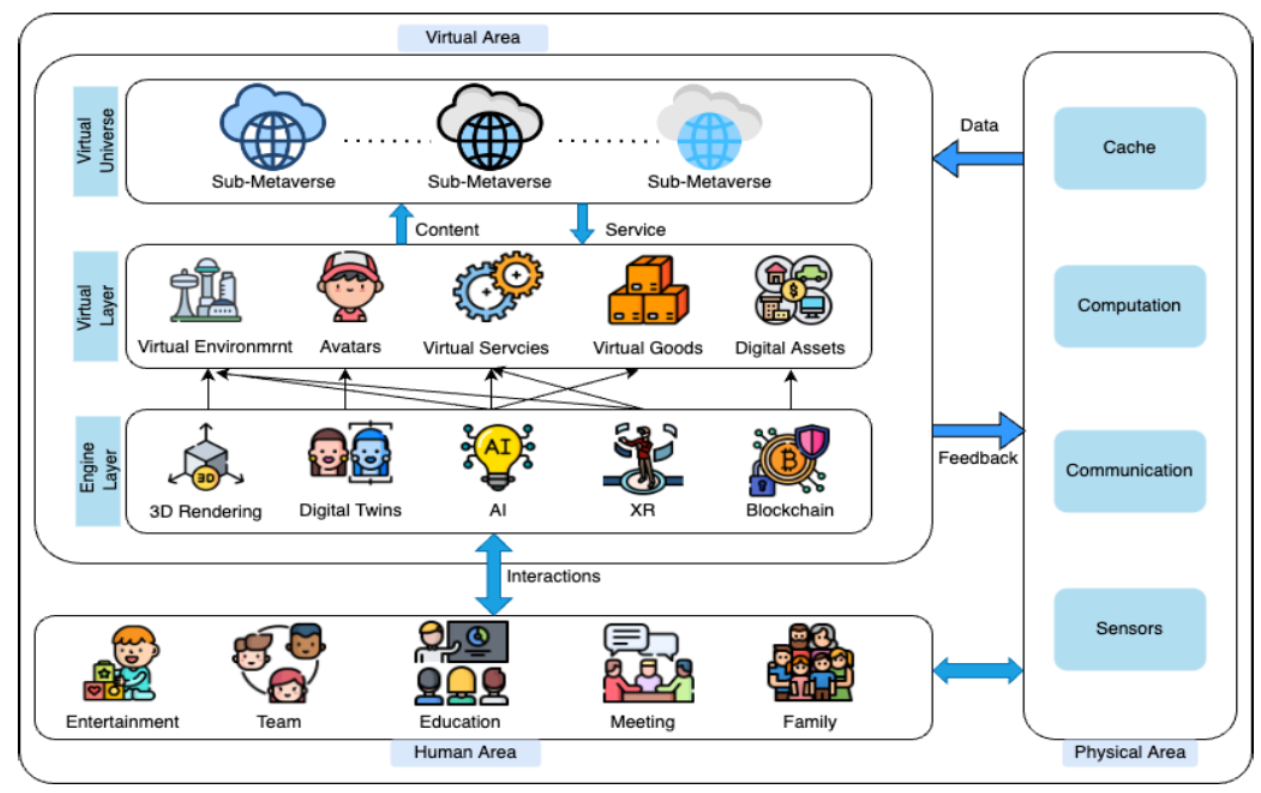
\includegraphics[width=\textwidth]{images/metaverse/metaverseAbstractArchitecture.png}
    \caption{Architektura Metaverse realizuje interakcje pomiędzy obszarem wirtualnym, obszarem ludzkim i obszarem fizycznym\cite{aSurveyofMobileEdgeComputingForMetaverse}}
    \label{abstractMetaverseArchitectureHumanVirtualPhisical}
\end{figure}

Kluczowe cechy metaverse:

\begin{itemize}
    \item Trwałość oznacza, istnienie niezależnie od fizycznej obecności użytkownika\cite{metaverseAFullDive}.
    \item Nieskończoność obsługiwanie niezliczonej liczby użytkowników i światów VR\cite{metaverseAFullDive}.
    \item Samowystarczalność oznacza, że użytkownicy mogą zarabiać w Metaverse i płacić za swoją użyteczność\cite{metaverseAFullDive}.
    \item Interoperacyjność pomaga użytkownikom przenosić ich wirtualne przedmioty, w tym awatary, z jednego projektu Metaverse do drugiego\cite{metaverseAFullDive}.
    \item Czas rzeczywisty pozwala użytkownikom cieszyć się doświadczeniami na żywo\cite{metaverseAFullDive}.
\end{itemize}


Metaverse ma być wciągającym wirtualnym światem, który płynnie łączy sferę fizyczną i cyfrową, umożliwiając użytkownikom interakcję, współpracę i angażowanie się w szereg działań we wspólnym wirtualnym środowisku. U podstaw tej rewolucyjnej koncepcji leży solidna infrastruktura, która służy jako szkielet, ułatwiając płynną łączność i interoperacyjność. Infrastruktura metaverse to ewoluująca, złożona sieć wzajemnie połączonych technologii, protokołów i ram, które współpracują ze sobą w celu stworzenia jednolitego i spójnego wirtualnego wszechświata\cite{metaverseInfrastructureIEEE}.

Infrastruktura ta obejmuje szeroką gamę komponentów, w tym szybkie sieci, potężne zasoby obliczeniowe, zaawansowane urządzenia sprzętowe i najnowocześniejsze platformy oprogramowania. Wykorzystuje ona najnowsze osiągnięcia w takich dziedzinach jak rzeczywistość wirtualna, rzeczywistość rozszerzona, blockchain i zdecentralizowane przetwarzanie danych, aby zapewnić wciągające i bezpieczne doświadczenie metawersji użytkownikom na całym świecie\cite{metaverseInfrastructureIEEE}.

\subsubsection{Architektura sieci w metawersji}

Architektura sieci w metaverse została zaprojektowana tak, aby wspierać płynne interakcje i komunikację w czasie rzeczywistym, umożliwiając użytkownikom angażowanie się w różne działania bez doświadczania opóźnień lub rozłączeń. Wykorzystuje ona zaawansowane protokoły i technologie sieciowe, które priorytetowo traktują niskie opóźnienia, wysoką przepustowość i wydajny transfer danych\cite{metaverseInfrastructureIEEE}.

Zdecentralizowane sieci odgrywają kluczową rolę w zwiększaniu łączności metaverse. Wykorzystując technologię blockchain i sieci peer-to-peer, infrastruktura metaverse ma na celu zmniejszenie zapotrzebowania na centralizacje zarządców lub pośredników. Takie podejście może zapewnić odporność, przejrzystość i demokratyczne zarządzanie, umożliwiając użytkownikom udział w rozwoju metawersji i procesach decyzyjnych\cite{metaverseInfrastructureIEEE}.

Przesyłanie danych i zarządzanie nimi w ramach infrastruktury metaverse jest ułatwione dzięki połączeniu tradycyjnych technologii sieciowych i nowych systemów rozproszonych. Szybkie sieci światłowodowe i łączność bezprzewodowa 5G/6G zapewniają przepustowość niezbędną do przesyłania bogatych treści multimedialnych i strumieni danych w czasie rzeczywistym. Jednocześnie zdecentralizowane rozwiązania pamięci masowej, takie jak rozproszone systemy plików i InterPlanetary File System \akronim{IPFS}, zapewniają bezpieczne i redundantne przechowywanie danych, umożliwiając efektywny dostęp do zasobów cyfrowych i ich wyszukiwania\cite{metaverseInfrastructureIEEE}.

Technologie przetwarzania na krawędzi (\english{Edge Computing}) mogą znacząco przyczynić się do zwiększenia wydajności infrastruktury metaverse. Przybliżając zasoby obliczeniowe do urządzeń brzegowych (takich jak zestawy słuchawkowe VR i okulary AR), przetwarzanie brzegowe zmniejsza opóźnienia i poprawia szybkość reakcji, zwiększając ogólne wrażenia użytkownika. Podejście to odciąża również scentralizowane serwery od zadań przetwarzania, rozkładając obciążenie obliczeniowe na całą sieć i zapewniając skalowalność w miarę wzrostu rozmiaru i złożoności metaverse\cite{metaverseInfrastructureIEEE}.

Technologie blockchain mogą odgrywać kluczową rolę w zwiększaniu bezpieczeństwa sieci w metawersji. Wykorzystując zdecentralizowane mechanizmy konsensusu i protokoły kryptograficzne, blockchain zapewnia integralność i niezmienność danych, chroniąc przed manipulacją i nieautoryzowanym dostępem. Dodatkowo, inteligentne kontrakty ułatwiają bezpieczne i przejrzyste interakcje, automatyzując złożone procesy i umożliwiając transakcje bez zaufania w ramach architektury metaverse i modelowania 3D\cite{metaverseInfrastructureIEEE}.

\subsubsection{Wymagania sprzętowe dla metawersji}

Aby uzyskać dostęp i w pełni doświadczyć metawersji, użytkownicy będą potrzebować specjalistycznego sprzętu, który może obsługiwać wciągające środowiska wirtualne i płynne interakcje. Podstawą tych wymagań sprzętowych są urządzenia komputerowe, takie jak komputery stacjonarne, konsole do gier lub wyspecjalizowane stacje robocze do rozwoju metaverse. Urządzenia te muszą posiadać wystarczającą moc obliczeniową, możliwości graficzne i zasoby pamięci, aby renderować szczegółowe środowiska 3D i obsługiwać złożone symulacje technologii metaverse\cite{metaverseInfrastructureIEEE}.

Infrastruktura metaverse w dużym stopniu wykorzystuje urządzenia rzeczywistości rozszerzonej i wirtualnej, aby zapewnić użytkownikom wciągające wrażenia. Zestawy VR, takie jak Oculus Rift, HTC Vive i PlayStation VR, przenoszą użytkowników do w pełni zrealizowanych wirtualnych światów, umożliwiając im interakcję z cyfrowymi obiektami i awatarami tak, jakby były prawdziwe. Urządzenia AR, takie jak Microsoft HoloLens i Magic Leap One, płynnie łączą elementy cyfrowe ze światem fizycznym, umożliwiając użytkownikom rozszerzenie otoczenia o wirtualne nakładki i interaktywne interfejsy\cite{metaverseInfrastructureIEEE}.

Zaawansowane jednostki przetwarzające, w tym wysokowydajne procesory graficzne \akronim{GPU} (\english{Graphics Processing Unit}) i wyspecjalizowane akceleratory, odgrywają kluczową rolę w zwiększaniu doznań płynących z metaverse. Komponenty te są odpowiedzialne za renderowanie złożonych środowisk 3D, symulację fizyki i przetwarzanie ogromnych ilości danych w czasie rzeczywistym. Dodatkowo, integracja sztucznej inteligencji i technologii uczenia maszynowego w infrastrukturze metaverse wymaga potężnych zasobów obliczeniowych, aby umożliwić inteligentne interakcje, przetwarzanie języka naturalnego i realistyczne awatary\cite{metaverseInfrastructureIEEE}.

Wraz z ciągłym rozwojem technologii, infrastruktura metaverse dostosowuje się do nowych technologii, które mogą jeszcze bardziej poprawić wrażenia użytkownika. Przykładowo, rozwój interfejsów mózg-komputer \akronim{BCI} (\english{Brain-Computer Interface}) i haptycznych urządzeń sprzężenia zwrotnego może zrewolucjonizować sposób interakcji użytkowników ze środowiskami wirtualnymi, umożliwiając bardziej intuicyjne i wciągające doświadczenia. Co więcej, postępy w dziedzinie obliczeń kwantowych i przetwarzania fotonicznego mogą potencjalnie zrewolucjonizować metawersję, zapewniając bezprecedensową moc obliczeniową a co za tym idzie możliwości przetwarzania danych\cite{metaverseInfrastructureIEEE}.

\subsubsection{Transakcje w metawersji}

Wirtualne waluty i technologia blockchain znajdują się w czołówce, jeśli chodzi o ułatwianie transakcji w metaverse. Te cyfrowe aktywa, często określane jako kryptowaluty lub tokeny, mogą służyć jako podstawowy środek wymiany towarów, usług i wirtualnych aktywów w wirtualnym środowisku metaverse. Wykorzystując zdecentralizowany i bezpieczny charakter technologii blockchain, te wirtualne waluty umożliwiają płynne, przejrzyste i pozbawione zaufania transakcje, eliminując potrzebę pośredników i zmniejszając koszty transakcji\cite{metaverseInfrastructureIEEE}.

Inteligentne kontrakty, które są samowykonalnymi umowami zakodowanymi w sieciach blockchain, mogą odgrywać kluczową rolę w automatyzacji i zabezpieczaniu transakcji w metaverse. Kontrakty te definiują zasady i warunki różnych umów, takich jak transfery aktywów, umowy o świadczenie usług i rozliczenia finansowe. Po wdrożeniu, inteligentne kontrakty wykonują się automatycznie, gdy spełnione są wcześniej określone warunki, zapewniając przejrzystość, wydajność i niezmienne prowadzenie dokumentacji dla wszystkich transakcji w ramach immersyjnego doświadczenia metaverse\cite{metaverseInfrastructureIEEE}.

Aktywami cyfrowymi i własnością intelektualną można zarządzać poprzez połączenie technologii blockchain i zdecentralizowanych rozwiązań w zakresie przechowywania. Tokeny niewymienialne \akronim{NFT} (\english{Non-Fungible Token}) mogą być wykorzystywane do reprezentowania unikalnych zasobów cyfrowych, takich jak wirtualne nieruchomości, dzieła sztuki, przedmioty kolekcjonerskie i przedmioty w grze. Tokeny te są przechowywane w sieciach blockchain, zapewniając łatwą weryfikację własności i pochodzenia. Ponadto zdecentralizowane systemy przechowywania plików, takie jak IPFS, umożliwiają bezpieczne i redundantne przechowywanie treści cyfrowych, zapewniając długowieczność i dostępność wirtualnych zasobów\cite{metaverseInfrastructureIEEE}.

Infrastruktura metaverse może ułatwiać wirtualne rynki i interakcje gospodarcze poprzez integrację zdecentralizowanych aplikacji \akronim{dApps} (\english{Decentralized application}) i zdecentralizowanych protokołów finansowych \akronim{DeFi} (\english{decentralized finance}). Platformy te umożliwiają użytkownikom kupowanie, sprzedawanie, handlowanie i inwestowanie w szeroką gamę wirtualnych aktywów, towarów i usług. Inteligentne kontrakty automatyzują i zarządzają tymi transakcjami, zapewniając uczciwość, przejrzystość i przestrzeganie wcześniej określonych zasad. Co więcej, zdecentralizowane autonomiczne organizacje \akronim{DAO} (\english{Decentralized autonomous organization}) pozwalają na zbiorowe podejmowanie decyzji i zarządzanie w ramach tych wirtualnych rynków, wspierając poczucie wspólnoty i współwłasności\cite{metaverseInfrastructureIEEE}.

\subsubsection{Ekosystem Metaverse}

\begin{figure}[!htbp]
    \centering
    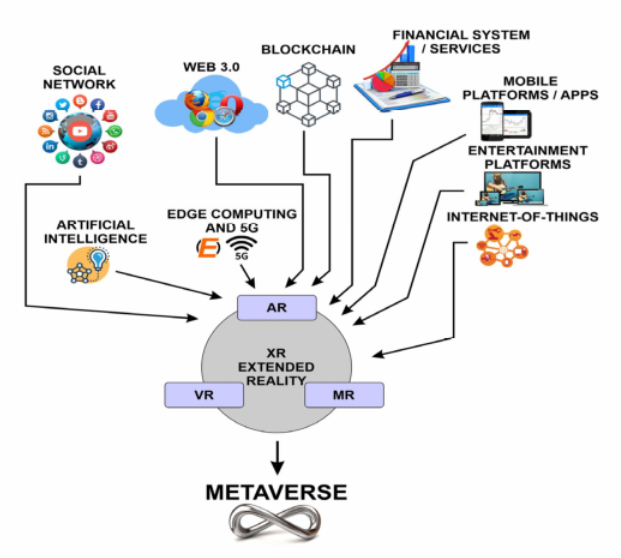
\includegraphics[width=\textwidth]{images/metaverse/metaverseEcosystem.png}
    \caption{Ekosystem Metaverse\cite{metaverseSecurityIssuesChallengesAndViableZTAModel}}
    \label{metaverseEcosystemImage}
\end{figure}

Metaverse umożliwia realizację kilku nowatorskich scenariuszy biznesowych w wielu różnych branżach. Połączenie tych technologii w połączeniu z nowymi rozwiązaniami pomoże zrealizować wizję metawersji w przyszłości. Rysunek \ref{metaverseEcosystemImage} przedstawia nadrzędny ekosystem technologiczny umożliwiający powstanie metawersji. Nie ulega wątpliwości, że technologie AR/VR/MR i XR stanowią podstawę metawersji, umożliwiając użytkownikom dostęp do wirtualnego świata 3D. W swojej najwcześniejszej iteracji metaverse może być zbiorem aplikacji Web 3.0 z XR-Skin zapewniającym ograniczone wrażenia VR. Oczekuje się, że sieci społecznościowe będą jednymi z pierwszych, które przeniosą się do metaverse, umożliwiając użytkownikom udostępnianie i konsumowanie treści immersyjnych wraz z Web 3.0, umożliwiając firmom oferowanie użytkownikom nowatorskich doświadczeń produktowych. Technologia blockchain zostanie szeroko wdrożona w metaverse, aby umożliwić realizację wizji zdecentralizowanych finansów i gospodarki twórców, które są nowymi tematami, głównie ze względu na bezpieczeństwo i prywatność, które oferują. Aplikacje i platformy mobilne mogą być kolejnymi, które migrują do metaverse, a następnie platformy rozrywkowe. Wreszcie, łączność 5G/6G, oferująca niskie opóźnienia, może być spoiwem, które płynnie połączy wszystkie elementy, podczas gdy Internet Rzeczy będzie łączył wszystkie urządzenia wraz z intensywnym wykorzystaniem sztucznej inteligencji, w tym inteligencji brzegowej, w celu zapewnienia spersonalizowanych doświadczeń\cite{metaverseSecurityIssuesChallengesAndViableZTAModel}. 
Można przewidzieć, że ekosystem metaverse przedstawiony na rysunku \ref{metaverseEcosystemImage} może przyjąć trzy potencjalne ścieżki ewolucji:

\begin{itemize}
    \item Zamknięty Metaverse: Dla niszowych aplikacji i przypadków użycia ograniczonych do użytku przez konkretną społeczność o wyspecjalizowanych potrzebach.
    \item Federacyjny: Zarządzana i obsługiwana przez dużą korporację z ekosystemem współpracujących partnerów, zewnętrznych dostawców i usługodawców dostarczających użytkownikom końcowym ujednolicone doświadczenie;  
    \item Otwarty Metaverse: Metawersja niesfederowana, nie kontrolowana przez żaden pojedynczy podmiot. O otwartej architekturze i społeczności deweloperów tworzących aplikacje/usługi dla użytkowników końcowych.
\end{itemize}



Prawdopodobnym jest, że ekosystem metaverse, jak pokazano na rysunku \ref{metaverseEcosystemImage}, może przyjąć trzy formy. Można oczekiwać, że wszystkie trzy modele będą współistnieć w takiej czy innej formie. Meta Facebooka jest doskonałym przykładem metawersji federacyjnej\cite{metaverseSecurityIssuesChallengesAndViableZTAModel}. 

Oczekuje się, że w przyszłości pojawią się inne modele, głównie napędzane przez sojusze biznesowe, fuzje i przejęcia. Jest prawdopodobne, że metaverse napotka kilka przeszkód na drodze do jego szerokiego przyjęcia. Niektóre z wyzwań stojących na drodze do realizacji pełnego potencjału koncepcji metaverse i jej przyjęcia obejmują:

\begin{itemize}
    \item Dostęp: Obecnie tylko przez zestawy okularów wirtualnej rzeczywistości, które nie są aktualnie powszechne
    \item Łatwość użytkowania: Użytkownicy uważają, że obecna wersja zestawów okularów wirtualnej rzeczywistości jest nieporęczna i trudna do noszenia przez długi czas
    \item Brak rozwiniętego ekosystemu: Niewiele aplikacji dostępnych na obecnych platformach VR
    \item Bezpieczeństwo i prywatność: Środowiska XR cierpią z powodu luk w zabezpieczeniach podstawowych technologii, w tym kwestii dotyczących prywatności użytkowników w wirtualnych światach. 
\end{itemize}

Podczas gdy oczekuje się, że postęp technologiczny rozwiąże kwestie dostępu i łatwości użytkowania w najbliższej przyszłości, kwestie bezpieczeństwa i prywatności muszą być budowane od podstaw podczas projektowania ekosystemu metaverse\cite{metaverseSecurityIssuesChallengesAndViableZTAModel}. 


\subsubsection{Podsumowanie}

Metawersja stanowi rewolucyjny skok w sposobie, w jaki ludzie postrzegają środowiska cyfrowe i wchodzą z nimi w interakcję, zacierając granice między sferą fizyczną i wirtualną. U podstaw tej koncepcji leży wiele koncepcji solidnej i zaawansowanej infrastruktury, która posłuży jako podstawa płynnej łączności, wciągających doświadczeń i nieograniczonych możliwości. 

W miarę jak metawersja będzie ewoluować i zyskiwać popularność, jej infrastruktura będzie odgrywać kluczową rolę w kształtowaniu przyszłości cyfrowych interakcji, handlu i kontaktów społecznych. Wykorzystując najnowocześniejsze technologie, takie jak blockchain, rzeczywistość wirtualna, rzeczywistość rozszerzona i zdecentralizowane przetwarzanie, infrastruktura metaverse umożliwia bezpieczne, przejrzyste i interoperacyjne przestrzenie wirtualne.

Pomyślne wdrożenie i rozwój metawersji będzie jednak również wymagać sprostania krytycznym wyzwaniom związanym z zarządzaniem, regulacjami, bezpieczeństwem i prywatnością. Współpraca między zainteresowanymi stronami, w tym deweloperami, decydentami i szerszą społecznością, jest niezbędna do ustanowienia skutecznych ram, które sprzyjają innowacjom, jednocześnie chroniąc użytkowników i utrzymując standardy etyczne.
\chapter{Implementacja}
\section{Wybrane narzędzia i technologie}
\subsection{Java}

\begin{figure}[!htbp]
    \centering
    
\includegraphics[width=0.2\textwidth]{images/javaLogo.png}
    \caption{Oficjalne logo języka Java}
    \label{fig:enter-label}
\end{figure}

Java jest to szeroko stosowany obiektowy język programowania i platforma oprogramowania, która działa na miliardach urządzeń. Zasady oraz składnia języka zostały oparte na językach \acronym{C} i \acronym{C++}. Java powstała aby udoskonalić i naprawić wiele błędnych konceptów wprowadzonych przez te języki. Jedną z głównych zalet tworzenia oprogramowania w Javie jest jej przenoszalność. Po napisaniu kodu programu na jednym urządzeniu można go łatwo przenieść na inne urządzenie o innej architekturze. Język ten został wynaleziony w 1995 roku przez Jamesa Goslinga z Sun Microsystems (później przejętego przez Oracle), główną ideą jego wynalezienia była możliwość, \definicja{"napisania raz, uruchomienia w dowolnym miejscu"}  (\english{write once, run anywhere}). Nowe i ulepszone narzędzia do tworzenia oprogramowania pojawiają się na rynku w nizwykłym tempie, wypierając dotychczasowe produkty, które kiedyś uważano za niezbędne. W świetle tej ciągłej rotacji, długowieczność Javy jest imponująca, prawie trzy dekady po jej stworzeniu, Java jest nadal najpopularniejszym językiem do tworzenia oprogramowania użytkowego\cite{javaIBM}\cite{javaDEV}.

Wszystkie języki programowania służą do komunikacji z maszynami. Sprzęt maszynowy reaguje tylko na komunikację elektroniczną. Języki programowania wysokiego poziomu, takie jak Java, działają jako pomost między językiem ludzkim a językiem sprzętu. Aby korzystać z języka Java programista musi mieć świadomość o dwóch poziomach abstrakcji pisanych programów: 

\begin{itemize}
    \item Język Java i \definicja{interfejsy \acronym{API} }(\english{application programming interface})
    \item Wirtualna maszyna Java \acronym{JVM} (\english{\termdef{Java Virtual Machine}})
\end{itemize}

Java definiuje składnię i semantykę języka. Obejmuje to podstawowe słownictwo i reguły używane do pisania algorytmów. 
Interfejsy API są ważnymi komponentami oprogramowania dołączonymi do platformy Java. Są to wstępnie napisane programy, które można podłączyć i odtworzyć istniejące funkcjonalności we własnym kodzie. Na przykład można użyć interfejsów API Java, aby uzyskać datę i godzinę, wykonać operacje matematyczne lub manipulować tekstem. Każdy kod aplikacji Java napisany przez programistę zazwyczaj łączy nowy i wcześniej istniejący kod z interfejsów API Java, bibliotek i frameworków\cite{frameworkDef}\cite{javaAmazon}\cite{javaDEV}.

Wirtualna maszyna Javy działa jako dodatkowa warstwa abstrakcji między platformą Java a sprzętem maszyny. Kod źródłowy Java może działać tylko na tych maszynach na których zainstalowano JVM. Kiedy po raz pierwszy opracowano języki programowania, dzieliły się one na dwie szerokie kategorie, w zależności od tego, w jaki sposób komunikowały się ze sprzętem: 

\begin{itemize}
    \item Kompilowany - program jest napisany w składni języka, a następnie kompilator tłumaczy cały kod na kod maszynowy. Skompilowany kod jest następnie uruchamiany na sprzęcie.
    \item Interpretowany - Dzięki interpreterom każda instrukcja kody wysokiego poziomu jest na bieżąco interpretowana na kod maszynowy. Napisane instrukcji są natychmiast uruchamiane przez sprzęt przed przejściem do następnej instrukcji
\end{itemize}

Język Java był pierwszym językiem, który połączył obie powyższe metody, przy użyciu JVM. Każdy plik programu jest najpierw kompilowany do kodu bajtowego (\english{bytecode}). Kod bajtowy Java może być uruchamiany tylko w maszynie JVM. Następnie JVM interpretuje kod bajtowy, aby uruchomić go na podstawowej platformie sprzętowej. Jeżeli aplikacja działa na komputerze z systemem Windows, maszyna JVM zinterpretuje ją dla systemu Windows. Natomiast jeżeli aplikacja uruchomiona jest na platformie open-source, takiej jak Linux, JVM zinterpretuje ją dla systemu Linux\cite{javaAmazon}\cite{javaDEV}.

\subsection{Maven}

\begin{figure}[htbp!]
    \centering
    
\includegraphics[width=0.5\textwidth]{images/mavenLogo.png}
    \caption{Logo programu Apache Maven\cite{mavenSite}.}
    \label{fig:enter-label}
\end{figure}

Maven słowo w języku jidysz oznacza gromadzenie wiedzy. Apache Maven to narzędzie do zarządzania projektami oprogramowania. Opiera się on na koncepcji \definicja{modelu obiektu projektu} (\acronym{POM} \english{Project Object Model}), Maven może zarządzać kompilacją, raportowaniem i dokumentacją projektu z centralnej informacji. Narzędzie to wykorzystywane jest do budowania i zarządzania dowolnym projektem opartym na Javie. Głównym źródłem informacji o projekcie jest plik \akronim{XML} (\english{Extensible Markup Language}) nazywany \acronym{POM}, w którym definiowana jest struktura projektu, sposób jego budowania oraz zależności jakie są wymagane do prawidłowego funkcjonowania programu. Maven podcza budowania aplikacji pobiera niezbędne biblioteki oraz inne zależności z globalnego repozytorium Maven Central.

\subsection{Spring boot}

\begin{figure}[!htbp]
    \centering
    
\includegraphics[width=0.5\textwidth]{images/springboot/springBootLogo.png}
    \caption{Logo frameworka Spring Boot \cite{springLogo}}
    \label{fig:enter-label}
\end{figure}


Spring boot jest jednym z najpopularniejszych frameworków języka Java wynalezionym przez Roda Johnsona w 2014 roku, który zapewnia funkcjonalność błyskawicznego wytwarzania aplikacji (\english{\definicja{Rapid Application Development \akronim{RAD}}}) polegającego na udostępnianiu programiście dużych możliwości prototypowania oraz dużego zestawu gotowych komponentów, narzędzi i modułów\cite{RADwiki}. Spring boot zbudowany jest na popularnym Java Spring Framework, aby zapewnić szybki dostęp do informacji podczas tworzenia projektu. Metodyka RAD jest dość łatwa do skonfigurowania i uruchomienia w internetowych i korporacyjnych aplikacjach przy użyciu języka Java. Najważniejszą rzeczą w tym frameworku jest jego prostota, do uruchomienia aplikacji wymagana jest minimalna konfiguracja, dzięki czemu tworzenie samodzielnych aplikacji opartych na Springu jest o wiele łatwiejsze\cite{springbootAnalysis}.

\subsubsection{Główne cechy Spring Boot Framework}

\begin{enumerate}
    \item Autokonfiguracja: Funkcja automatycznej konfiguracji Spring Boot automatycznie konfiguruje aplikację Spring na podstawie dodanych zależności. Na przykład, jeżeli została dołączona zależność spring-boot-starter-web, automatycznie zostaje skonfigurowany serwer Tomcat i Spring \acronym{MVC} (\english{Model-View-Controller})\cite{springbootFeatures}.
    \item Samodzielna aplikacja: Aplikacje Spring Boot mogą być uruchamiane jako samodzielne aplikacje Java. Jest to ułatwione dzięki osadzeniu serwera HTTP (takiego jak Tomcat, Jetty lub Undertow) bezpośrednio w aplikacji, co ułatwia jej wdrożenie\cite{springbootFeatures}.
    \item Funkcje gotowe do produkcji: Spring Boot zawiera kilka wbudowanych funkcji ułatwiających uruchamianie aplikacji w środowisku produkcyjnym. Obejmują one kontrole kondycji, metryki, monitorowanie aplikacji i konfigurację zewnętrzną\cite{springbootFeatures}.
    \item Konwencja ponad konfiguracją: Spring Boot kieruje się filozofią zapewniania rozsądnych wartości domyślnych, aby zminimalizować ilość wymaganej konfiguracji. Jednak nadal pozwala na zastąpienie tych domyślnych ustawień, gdy jest to konieczne\cite{springbootFeatures}.
    \item Rozwój mikrousług: Spring Boot jest szeroko stosowany do tworzenia mikrousług ze względu na jego lekki i modułowy charakter. Zapewnia wbudowane serwery, łatwą integrację ze środowiskami chmurowymi i wsparcie dla systemów rozproszonych\cite{springbootFeatures}.
    \item Startery Spring Boot: Startery to zestaw wygodnych deskryptorów zależności, które można dołączyć do aplikacji. Na przykład spring-boot-starter-data-jpa zawiera zależności do używania \acronym{JPA} (\english{Java Persistence \acronym{API}}) ze Spring Data\cite{springbootFeatures}.
    \item Wbudowane serwery: Spring Boot obsługuje wbudowane serwery, takie jak Tomcat, Jetty i Undertow, umożliwiając pakowanie aplikacji jako plików \acronym{JAR} (\english{Java Archive}) i uruchamianie ich niezależnie od zewnętrznych serwerów\cite{springbootFeatures}.
    \item Spring Initializr: Spring Initializr to narzędzie internetowe do szybkiego generowania struktury projektu Spring Boot. Pozwala programistom wybrać żądane zależności projektu i wygenerować szkielet projektu\cite{springbootFeatures}.
    \item Obszerna dokumentacja i wsparcie społeczności: Spring Boot jest dobrze udokumentowany i ma dużą i aktywną społeczność, która przyczynia się do jego ciągłego rozwoju i wsparcia\cite{springbootFeatures}.
    \item Korzystając ze Spring Boot, programiści mogą usprawnić tworzenie aplikacji opartych na Spring, wykorzystując potężne funkcje frameworka w celu zmniejszenia ilości standardowego kodu i wysiłku związanego z konfiguracją\cite{springbootFeatures}.
\end{enumerate}

\begin{figure}[!h]
    \centering
    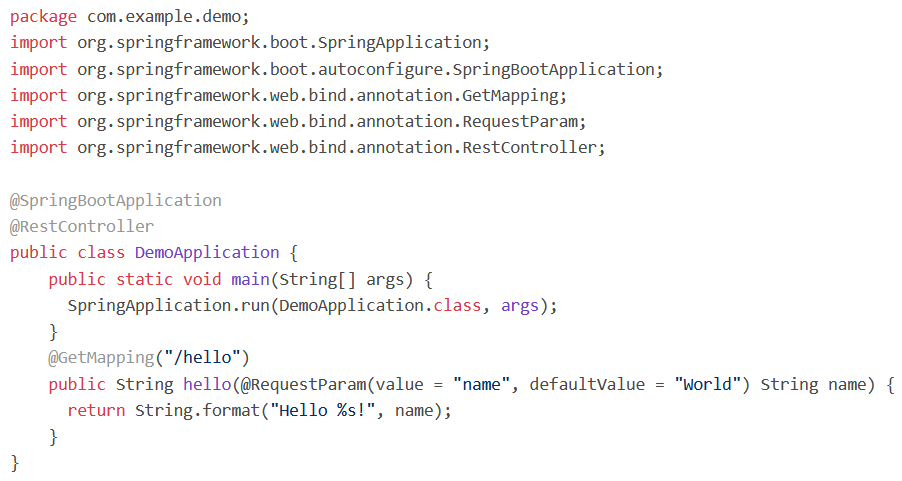
\includegraphics[width=0.8\textwidth]{images/springboot/exampleJavaSpringBootProgram.png}
    \caption{Przykładowy program java napisany z wykorzystaniem frameworku Springboot\cite{springJavaExampleProgram}}
    \label{fig:enter-label}
\end{figure}

Powyższy program składa się z głównej klasy aplikacji z adnotacją @SpringBootApplication, która wskazuje klasę konfiguracyjną, która deklaruje jedną lub więcej metod @Bean, a także uruchamia automatyczną konfigurację i skanowanie komponentów. Klasa DemoApplication zawiera główną metodę, która jest punktem wejścia aplikacji. Metoda SpringApplication.run uruchamia cały framework Spring.
Dodatkowo klasa jest opatrzona adnotacją @RestController, wskazującą, że jest to kontroler sieciowy, w którym każda metoda zwraca obiekt domeny zamiast widoku. Metoda hello jest mapowana do punktu końcowego /hello przy użyciu adnotacji @GetMapping, co pozwala jej obsługiwać żądania HTTP GET. Metoda ta przyjmuje nazwę parametru żądania z domyślną wartością „World” i zwraca wiadomość powitalną.

\subsection{Netflix Eureka}

\begin{figure}[!htbp]
    \centering
    
\includegraphics[width=0.7\textwidth]{images/netflixEureka/netflixEurekaLogo.png}
    \caption{Spring Cloud Netflix\cite{netflixEurekaMedium}}
    \label{fig:enter-label}
\end{figure}

Odnajdywanie usług jest jednym z kluczowych założeń zarchitektury opartej na mikrousługach. Próba ręcznego konfigurowania każdego klienta lub jakiejś formy usługodawcy może być trudna do wykonania i ulotna. Usługa odkrywania (\english{Service Discovery}) jest to proces automatycznego odnajdywania i wykrywania usług i urządzeń w sieci. Serwer Eureka to usługa oparta na \akronim{REST} (\english{Representational State Transfer}), która jest wykorzystywana głównie w chmurze Amazon \akronim{AWS} (\english{Amazon Web Services}) do lokalizowania usług w celu równoważenia obciążenia i przełączania awaryjnego serwerów. Eureka jest również dostarczana z komponentem klienckim opartym na Javie, Eureka Client, który znacznie ułatwia komunikacje z usługą\cite{netflixEurekaArticleWang}\cite{netflixEurekaGithub}\cite{springEureka}\cite{netflixEurekaManual}.

\begin{figure}[!htbp]
    \centering
    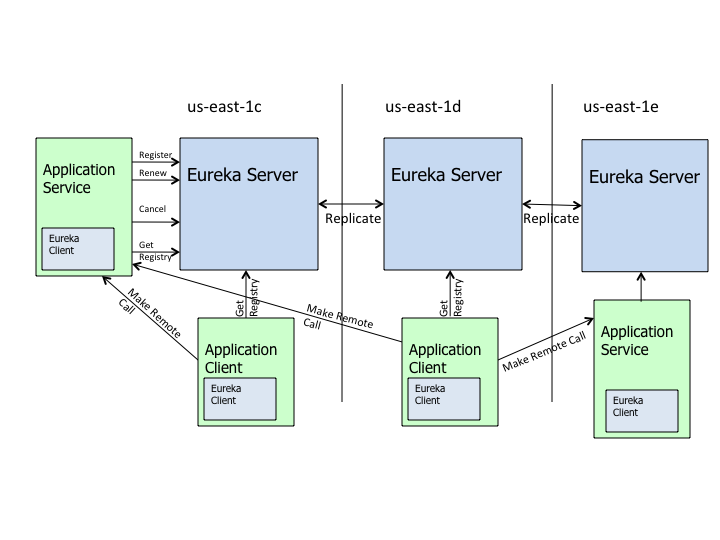
\includegraphics[width=\textwidth, trim={0 4cm 0 0}]{images/netflixEureka/eureka_architecture.png}
    \caption{przykładowa architektura klastra usług Eureka w Netflixie\cite{netflixEurekaGithub}}
    \label{fig:enter-label}
\end{figure}

Powyższa architektura przedstawia sposób, w jaki Eureka jest wdrażana w Netflixie i jest to typowy sposób jej uruchamiania. Na każdy region przypada jedna usługa (bądź też klaster usług) Eureka, w którym rejestrują się instancje z tego regionu, w którym jest uruchomiona. Usługi rejestrują się w serwerze Eureka, a następnie co 30 sekund wysyłają bicie serca (\english{heartbeats}), aby odnowić swoje dzierżawy. Jeżeli usługa nie może odnowić dzierżawy kilka razy, jest ona usuwana z rejestru serwera w ciągu około 90 sekund. Informacje o rejestracji i odnowieniach są replikowane do wszystkich węzłów Eureka w klastrze. Klienci z dowolnej strefy mogą wyszukiwać informacje w rejestrze, aby zlokalizować swoje usługi (które mogą znajdować się w innej strefie niż klient) następnie po otrzymaniu informacji o szukanej instancji, klient wykonuje połączenie do usługi\cite{netflixEurekaArticleWang}\cite{netflixEurekaGithub}\cite{springEureka}\cite{netflixEurekaManual}.

\subsection{Docker}

\begin{figure}[!htbp]
    \centering
    
\includegraphics[width=0.5\textwidth]{images/Docker_logo.png}
    \caption{Logo marki Docker \cite{DockerMedia}}
    \label{fig:enter-label}
\end{figure}

W przeszłości aplikacje były zazwyczaj wdrażane na serwerach fizycznych lub maszynach wirtualnych. Przed wdrożeniem aplikacji należy skonfigurować niezbędną infrastrukturę. Obejmowało to instancję systemu operacyjnego, wszelkich zależności wymaganych przez aplikację i skonfigurowanie wszystkiego by ze sobą współpracowało w prawidłowy sposób. Było to czasochłonne i skomplikowane, zwłaszcza gdy próbowało się odtworzyć dokładnie to środowisko, dla którego aplikacja została stworzona.
Maszyny wirtualne stanowiły pod tym względem znaczącą przewagę nad serwerami fizycznymi. Umożliwiały one programistom oddzielenie tworzonego oprogramowania od bazowego systemu. Dodatkowo, oferowały one deweloperom łatwo dostępne środowisko, które mogli wykorzystywać do rozwoju i testowania, oddzielone od głównego systemu operacyjnego. Jednak maszyny wirtualne nadal posiadały swój własny zestaw wyzwań\cite{dockerContenerizationKeyAndUseCases}. 

Jednym z nich głównych problemów jest to, że wymagały one pełnej kopi systemu operacyjnego. Oznacza to, że były one stosunkowo duże i zajmowały dużo zasobów. Z tego powodu uruchamianie wielu maszyn wirtualnych na tym samym serwerze fizycznym było dość kosztowne. Kosztowne z dwóch perspektyw. Nie tylko uruchomienie setek maszyn wirtualnych kosztowało znaczną ilość pieniędzy, ale także wymagało dużej ilości zasobów, takich jak rdzenie procesora, pamięć \acronym{RAM} (\english{Random Access Memory}) i przestrzeń dyskową. Co więcej, trudno było skalować aplikacje w poziomie, oznacza to dodanie większej ilości replik aplikacji w celu obsłużenia zwiększonego ruchu, liczny użytkowników czy obciążenia pracy danej repliki\cite{dockerContenerizationKeyAndUseCases}.

Konteneryzacja oferuje natomiast szereg korzyści, które pozwalają sprostać tym wyzwaniom. Dzięki konteneryzacji, deweloperzy mogą spakować swoje aplikacje i ich zależności w jednym kontenerze. Kontener ten może natomiast dostarczyć i wdrożyć na dowolnej platformie, która je obsługuje. Ułatwia to wdrożenie i uruchamianie aplikacji w rożnych środowiskach. Konteneryzacja oferuje spójne i niezawodne działanie aplikacji na różnych platformach, niezależnie od tego czy jest to serwer fizyczny maszyna wirtualna w chmurze, czy też system operacyjny Windows lub Linux\cite{dockerContenerizationKeyAndUseCases}\cite{dockerOverview}. 

Dodatkowymi atutami konteneryzacji są:

\begin{itemize}
    \item Przenaszalność: Konteneryzowanie aplikacji może łatwo przenieść między różnymi środowiskami. Na przykład, można je łatwo przenieść z laptopa dewelopera do środowiska przejściowego lub produkcyjnego. Nie trzeba martwić się o różne konfiguracje między laptopem a serwerem, na którym zostanie wdrożony kontener\cite{dockerContenerizationKeyAndUseCases}\cite{dockerOverview}.
    
    \item Izolacja: Kontenery zapewniają warstwę izolacji między aplikacją a systemem hosta. Jest to coś w rodzaju bariery ochronnej, która pomaga zapobiegać konfliktom między różnymi aplikacjami lub zależnościami. Każdy kontener działa w swoim własnym, odizolowanym środowisku. Oznacza to, że jest mniej prawdopodobne, że wpłyną na niego inne aplikacje lub procesy działające na tej samej maszynie hosta. W związku z tym znacznie trudniej jest aplikacjom w kontenerach negatywnie wpływać na siebie nawzajem lub na system hosta. Pliki w systemie hosta i w innych kontenerach pozostaną nienaruszone, ponieważ aplikacja nie może uzyskać dostępu do plików spoza własnego środowiska\cite{dockerContenerizationKeyAndUseCases}\cite{dockerOverview}.

    \item Wydajność zasobów: Kontenery umożliwiają uruchamianie wielu odizolowanych aplikacji w tym samym systemie hosta. Nie trzeba przydzielać zasobów do każdej z nich z osobna (jak ma to miejsce w przypadku maszyn wirtualnych). Skutkuje to znacznym zmniejszeniem wykorzystania zasobów i kosztów. Ta zaleta jest szczególnie korzystna w środowiskach chmurowych, gdzie opłaty są często oparte na wykorzystaniu zasobów\cite{dockerContenerizationKeyAndUseCases}\cite{dockerOverview}.

    \item Łatwe pakowanie, dostarczanie i wdrażanie: Dla dewelopera spakowanie aplikacji do obrazu kontenera jest prostym procesem. Następnie deweloper może przesłać zbudowany obraz do rejestru kontenerów, który działa jako scentralizowany serwer do dystrybucji obrazu innym osobom. W ten sposób inne osoby mogą w prosty sposób pobrać zbudowany obraz na swoje urządzenie i go uruchomić\cite{dockerContenerizationKeyAndUseCases}\cite{dockerOverview}.
\end{itemize}

W 2013 roku pojawił się Docker, który sprawił że korzystanie z kontenerów stało się niezwykle proste. Dzięki Dockerowi można było tworzyć obrazy, przesyłać je do repozytorium, uruchamiać kontenery, łączyć je w sieci i wykonywać wiele innych zadań związanych z kontenerami. Oznacza to, że wystarczy użyć tylko jednego narzędzia aby obsłużyć wszystkie potrzeby związane z kontenerami. W rezultacie kontenery stały się głównym nurtem i zyskały ogromną popularność\cite{dockerContenerizationKeyAndUseCases}\cite{dockerOverview}.

\subsubsection{Docker Compose}

Docker Compose to narzędzie do definiowania i uruchamiania aplikacji wielokontenerowych. Jest to klucz do odblokowania usprawnionego i wydajnego środowiska programowania i wdrażania.
Compose upraszcza kontrolę nad całym stosem aplikacji, ułatwiając zarządzanie usługami, sieciami i wolumenami w jednym, zrozumiałym pliku konfiguracyjnym \akronim{YAML} (\english{YAML Ain’t Markup Language}). Następnie za pomocą jednego polecenia można utworzyć i uruchomić wszystkie usugi z pliku konfiguracyjnego. Compose działa we wszystkich środowiskach: produkcyjnym, przejściowym, deweloperskim, testowym, a także w przepływach pracy \akronim{CI} (\english{Continuous Integration})\cite{dockerComposeAStudyMultiContainerSystem}\cite{dockerComposeOverview}\cite{dockerComposePaterns}. 

Posiada również polecenia do zarządzania całym cyklem życia aplikacji: 
\begin{itemize}
    \item Uruchamianie, zatrzymywanie i przebudowywanie stosu usług
    \item Wyświetlenie stanu uruchomionych aplikacji
    \item Przesyłanie strumieniowe danych wyjściowych dziennika uruchomionych usług
    \item Uruchamianie jednorazowego polecenia w określonym kontenerze
\end{itemize}

\subsection{Środowisko programistyczne - InteliJ}
\subsection{Insomnia}
\subsection{Logstash Logback Encoder}




\newpage
% Temporarily change the margins for this page
\newgeometry{
  left=0.5in,
  right=0.5in,
  top=1.5in,
  bottom=1in,
}
\section{Elementy tworzonego systemu}
\begin{figure}[!htbp]
    \centering
    \includesvg[scale=0.5,angle=90]{schemas/master-Dev.drawio.svg}
    \caption{Schemat tworzonego systemu}
    \label{fig:enter-label}
\end{figure}

% Restore the original margins
\restoregeometry
\newpage

\subsection{Producent}
\subsection{Rejestr usług}
\subsection{Węzeł protokołu}
\subsubsection{Podsystem monitoringu producentów}
\subsubsection{Podsystem propozycji zasobów}

\section{Uruchomienie środowiska}
\chapter{Monitoring}

\chapter{Kierunki rozwoju}
\chapter{Podsumowanie}



%--------------------------------------
% Literatura
%--------------------------------------

\bibliographystyle{IEEEtran}{\raggedright\sloppy\small\bibliography{bibliografia}}

%--------------------------------------
% Spis ilustracji
%--------------------------------------
\newpage
\listoffigures


%--------------------------------------
% Dodatki
%--------------------------------------

\cleardoublepage\appendix%

%-------------------------------------
% Informacja o prawach autorskich
%--------------------------------------

\ppcolophon

\end{document}
